Joel le va a mandar un sobre grande por correo a su primo. El sobre contiene fotografías, así que no quiere doblarlo.
La ranura del buzón tiene las dimensiones que se muestran a continuación en la figura \ref{fig:proverb_pitagoras_02}. La línea punteada muestra la parte más ancha de la ranura.
\begin{figure}[H]
    \begin{center}
        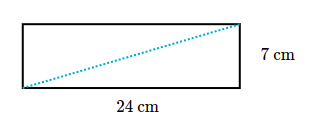
\includegraphics[width=0.5\textwidth]{../images/proverb_pitagoras_02.png}
    \end{center}
    \caption{}
    \label{fig:proverb_pitagoras_02}
\end{figure}
\textbf{¿Cuál es el ancho máximo de la ranura del buzón?}\\


\begin{solutionbox}{7cm}
    Podemos usar el teorema de Pitágoras para obtener $x$.
    La ecuación del teorema de Pitágoras es:
    \[c^2=a^2+b^2\]
    donde $a$ y $b$ son las longitudes de los dos catetos del triángulo y $c$ es la longitud de la hipotenusa.
    En este caso, $a=7$, $b=24$ y $c=x$.
    \begin{align*}
        x^2 & =7^2+24^2   \\
        x^2 & =625        \\
        x   & =\sqrt{625} \\
        x   & =25
    \end{align*}
    El ancho máximo de la ranura del correo es 25 cm.
\end{solutionbox}